
\subsection{Fit at the tract level}

The tract distributions are fitted to every indicator the ADRH publishes for the tract, so comparing them with those indicators measures the quality of the fit rather than its predictive accuracy. For the \ValTracts{} tracts with a GB2 fit, all averages and regressions below weight tracts by population. The fitted median lies inside the published \texteuro 700 interval in \FitMedInBinPct{}\% of tracts; fitted and published means differ by \FitMeanAbsErr{}\% on average, Gini coefficients by \FitGiniAbsErr{} points and P80/P20 ratios by \FitPAbsErr{}\%, the latter partly because published ratios come from rounded percentiles. The nine shares differ from the published ones by \FitShareMAE{} percentage points on average.

\paragraph{Mean-to-median ratio} The ratio of the mean to the median summarizes the skewness of each tract's distribution. Figure \ref{fig:skew} plots the observed $\ln(\bar y_j / \tilde m_j)$, where $\bar y_j$ and $\tilde m_j$ are the published mean and median, against its fitted value. A regression of observed on fitted values has a slope of \ValSkewSlope{} ($R^2 = \ValSkewRsq{}$).

\begin{figure}[!htb]
\begin{center}
\caption{Mean-to-median ratio: observed and fitted}
\label{fig:skew}
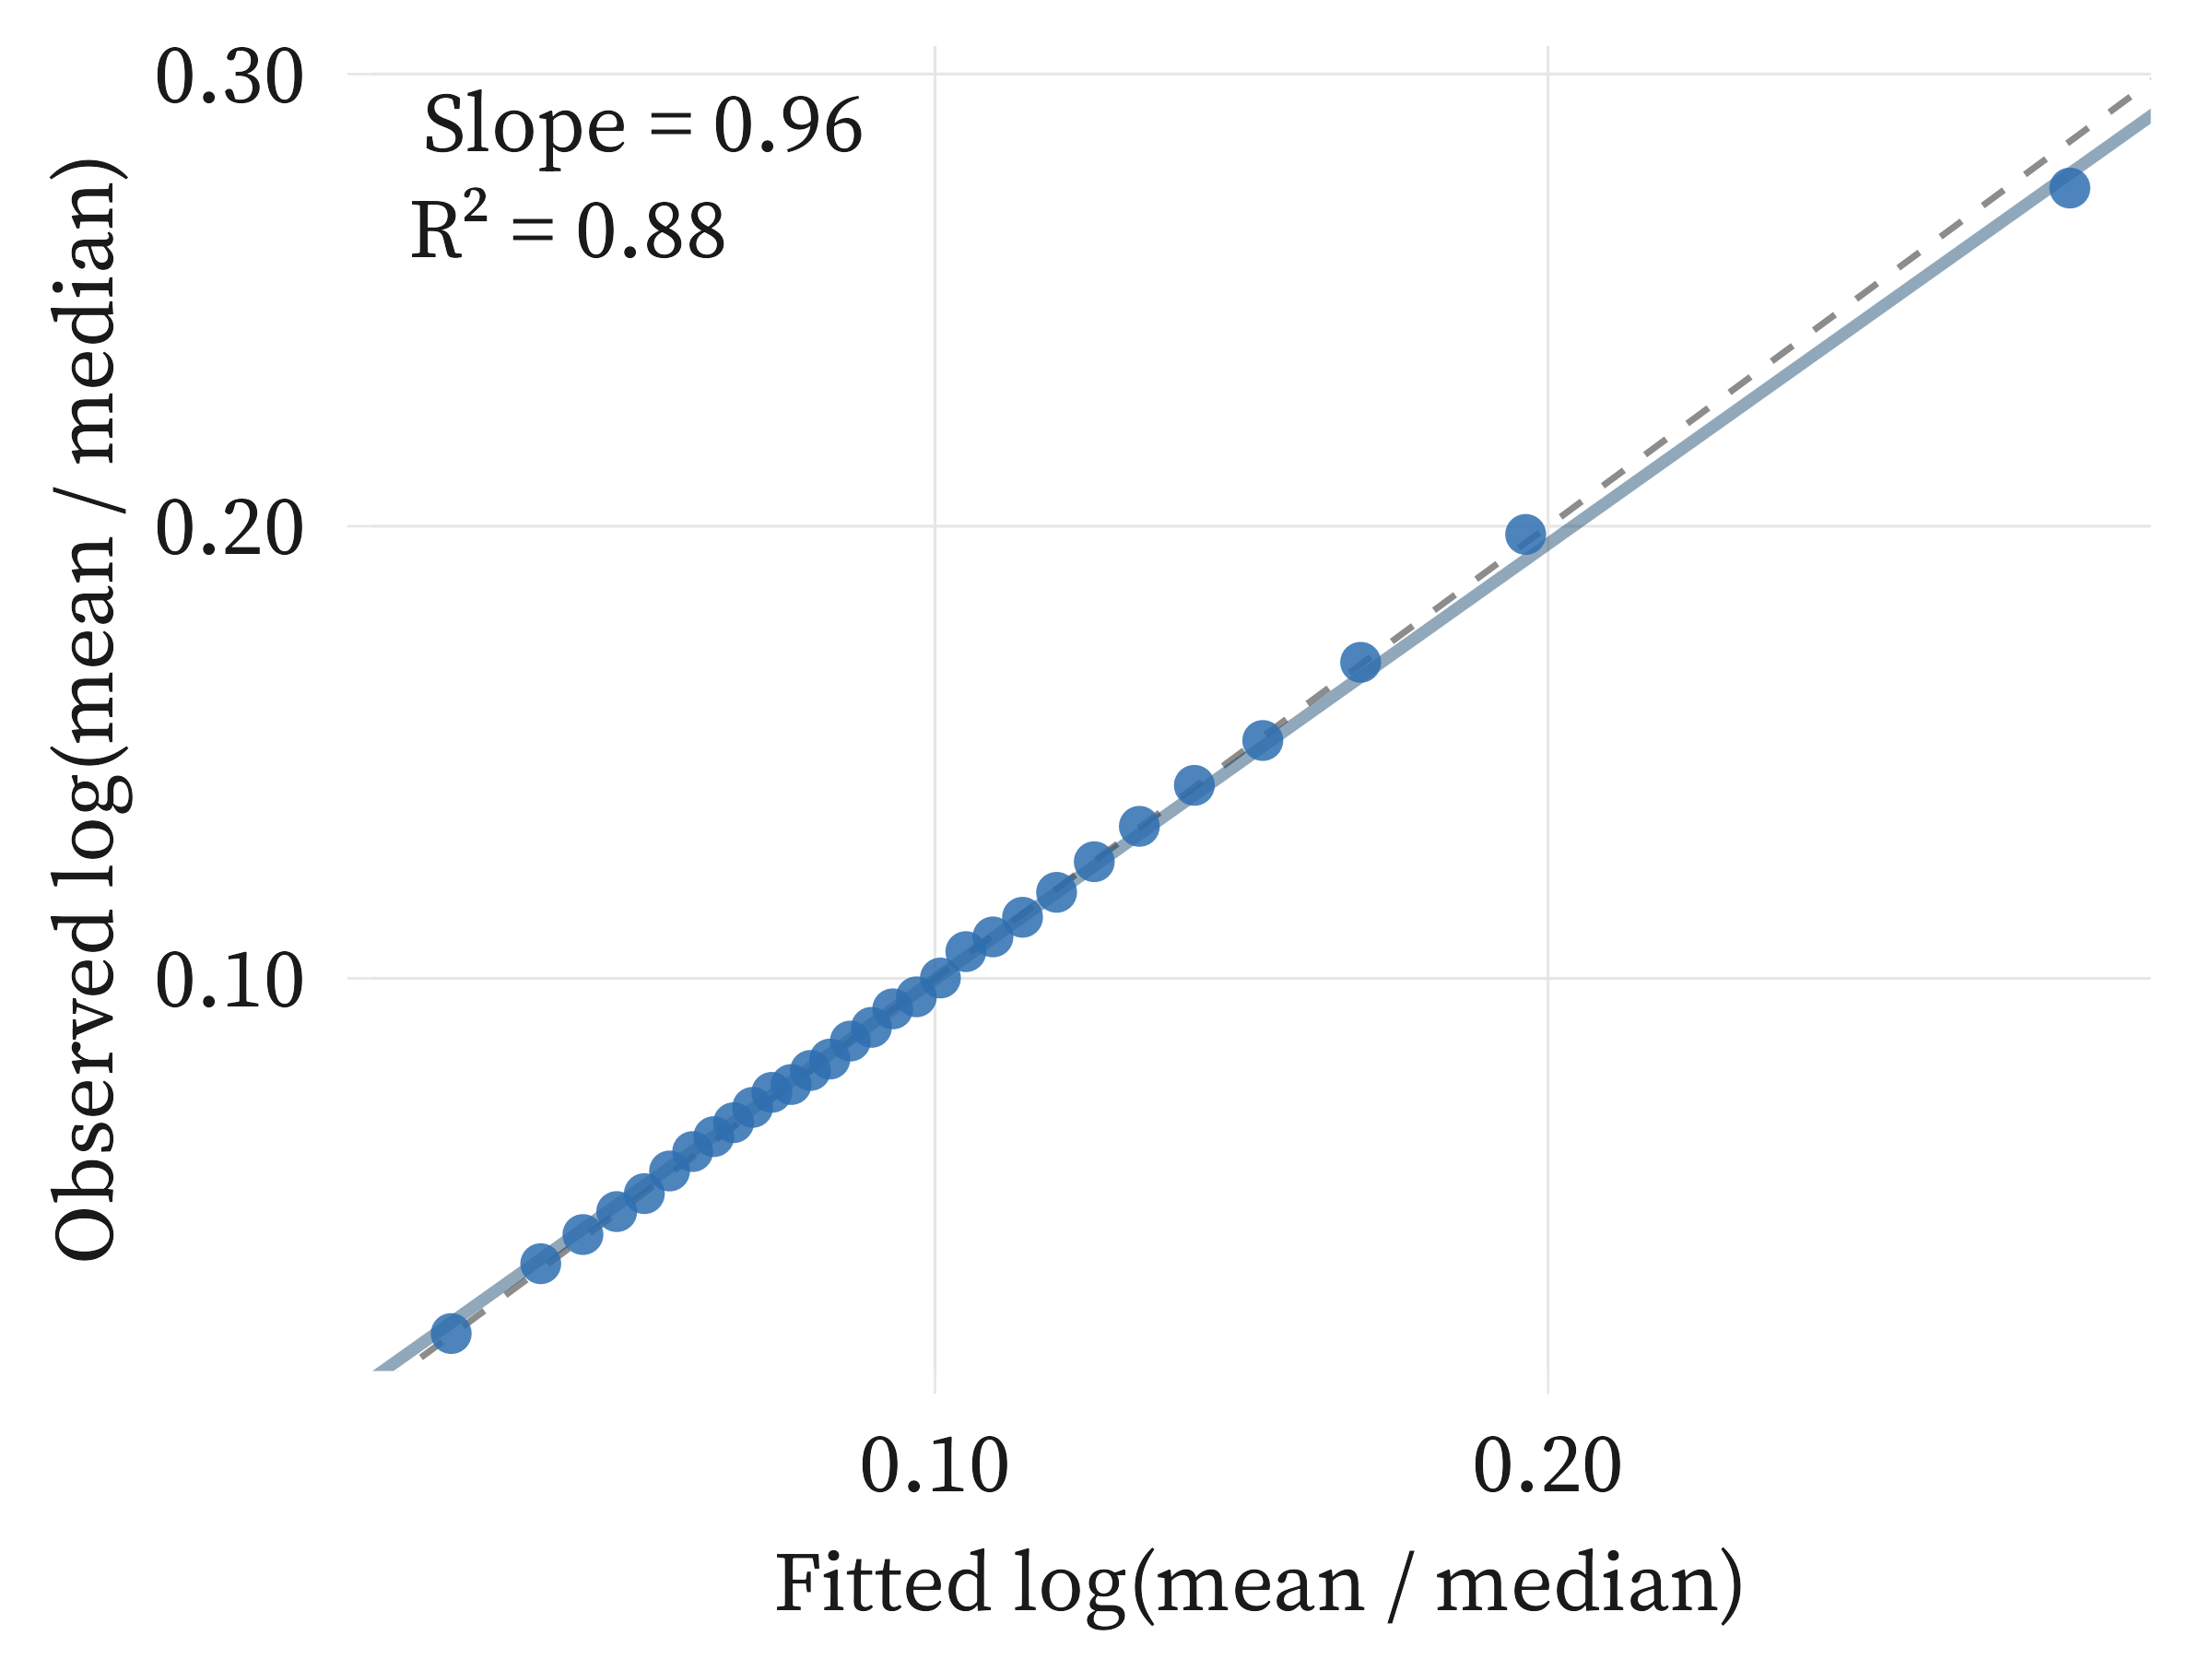
\includegraphics[width=0.55\textwidth]{output/fig_validation_skew.png}
\end{center}
\begin{fignotes2}
\textbf{Notes:} Binned scatter plot of the observed $\ln(\text{mean}/\text{median})$ of income per consumption unit against its value under the tract's fitted GB2. Tracts are grouped into 30 bins of equal population. The solid line is the population-weighted regression of observed on fitted values over all tracts; the dashed line is the 45-degree line. Source: INE, ADRH (\BaseYear{}), and author's calculations.
\end{fignotes2}
\end{figure}

\paragraph{P80/P20 ratio} Figure \ref{fig:p80p20} does the same for the P80/P20 ratio. A regression of observed on fitted ratios has a slope of \ValPSlope{} ($R^2 = \ValPRsq{}$).

\begin{figure}[!htb]
\begin{center}
\caption{P80/P20 ratio: observed and fitted}
\label{fig:p80p20}
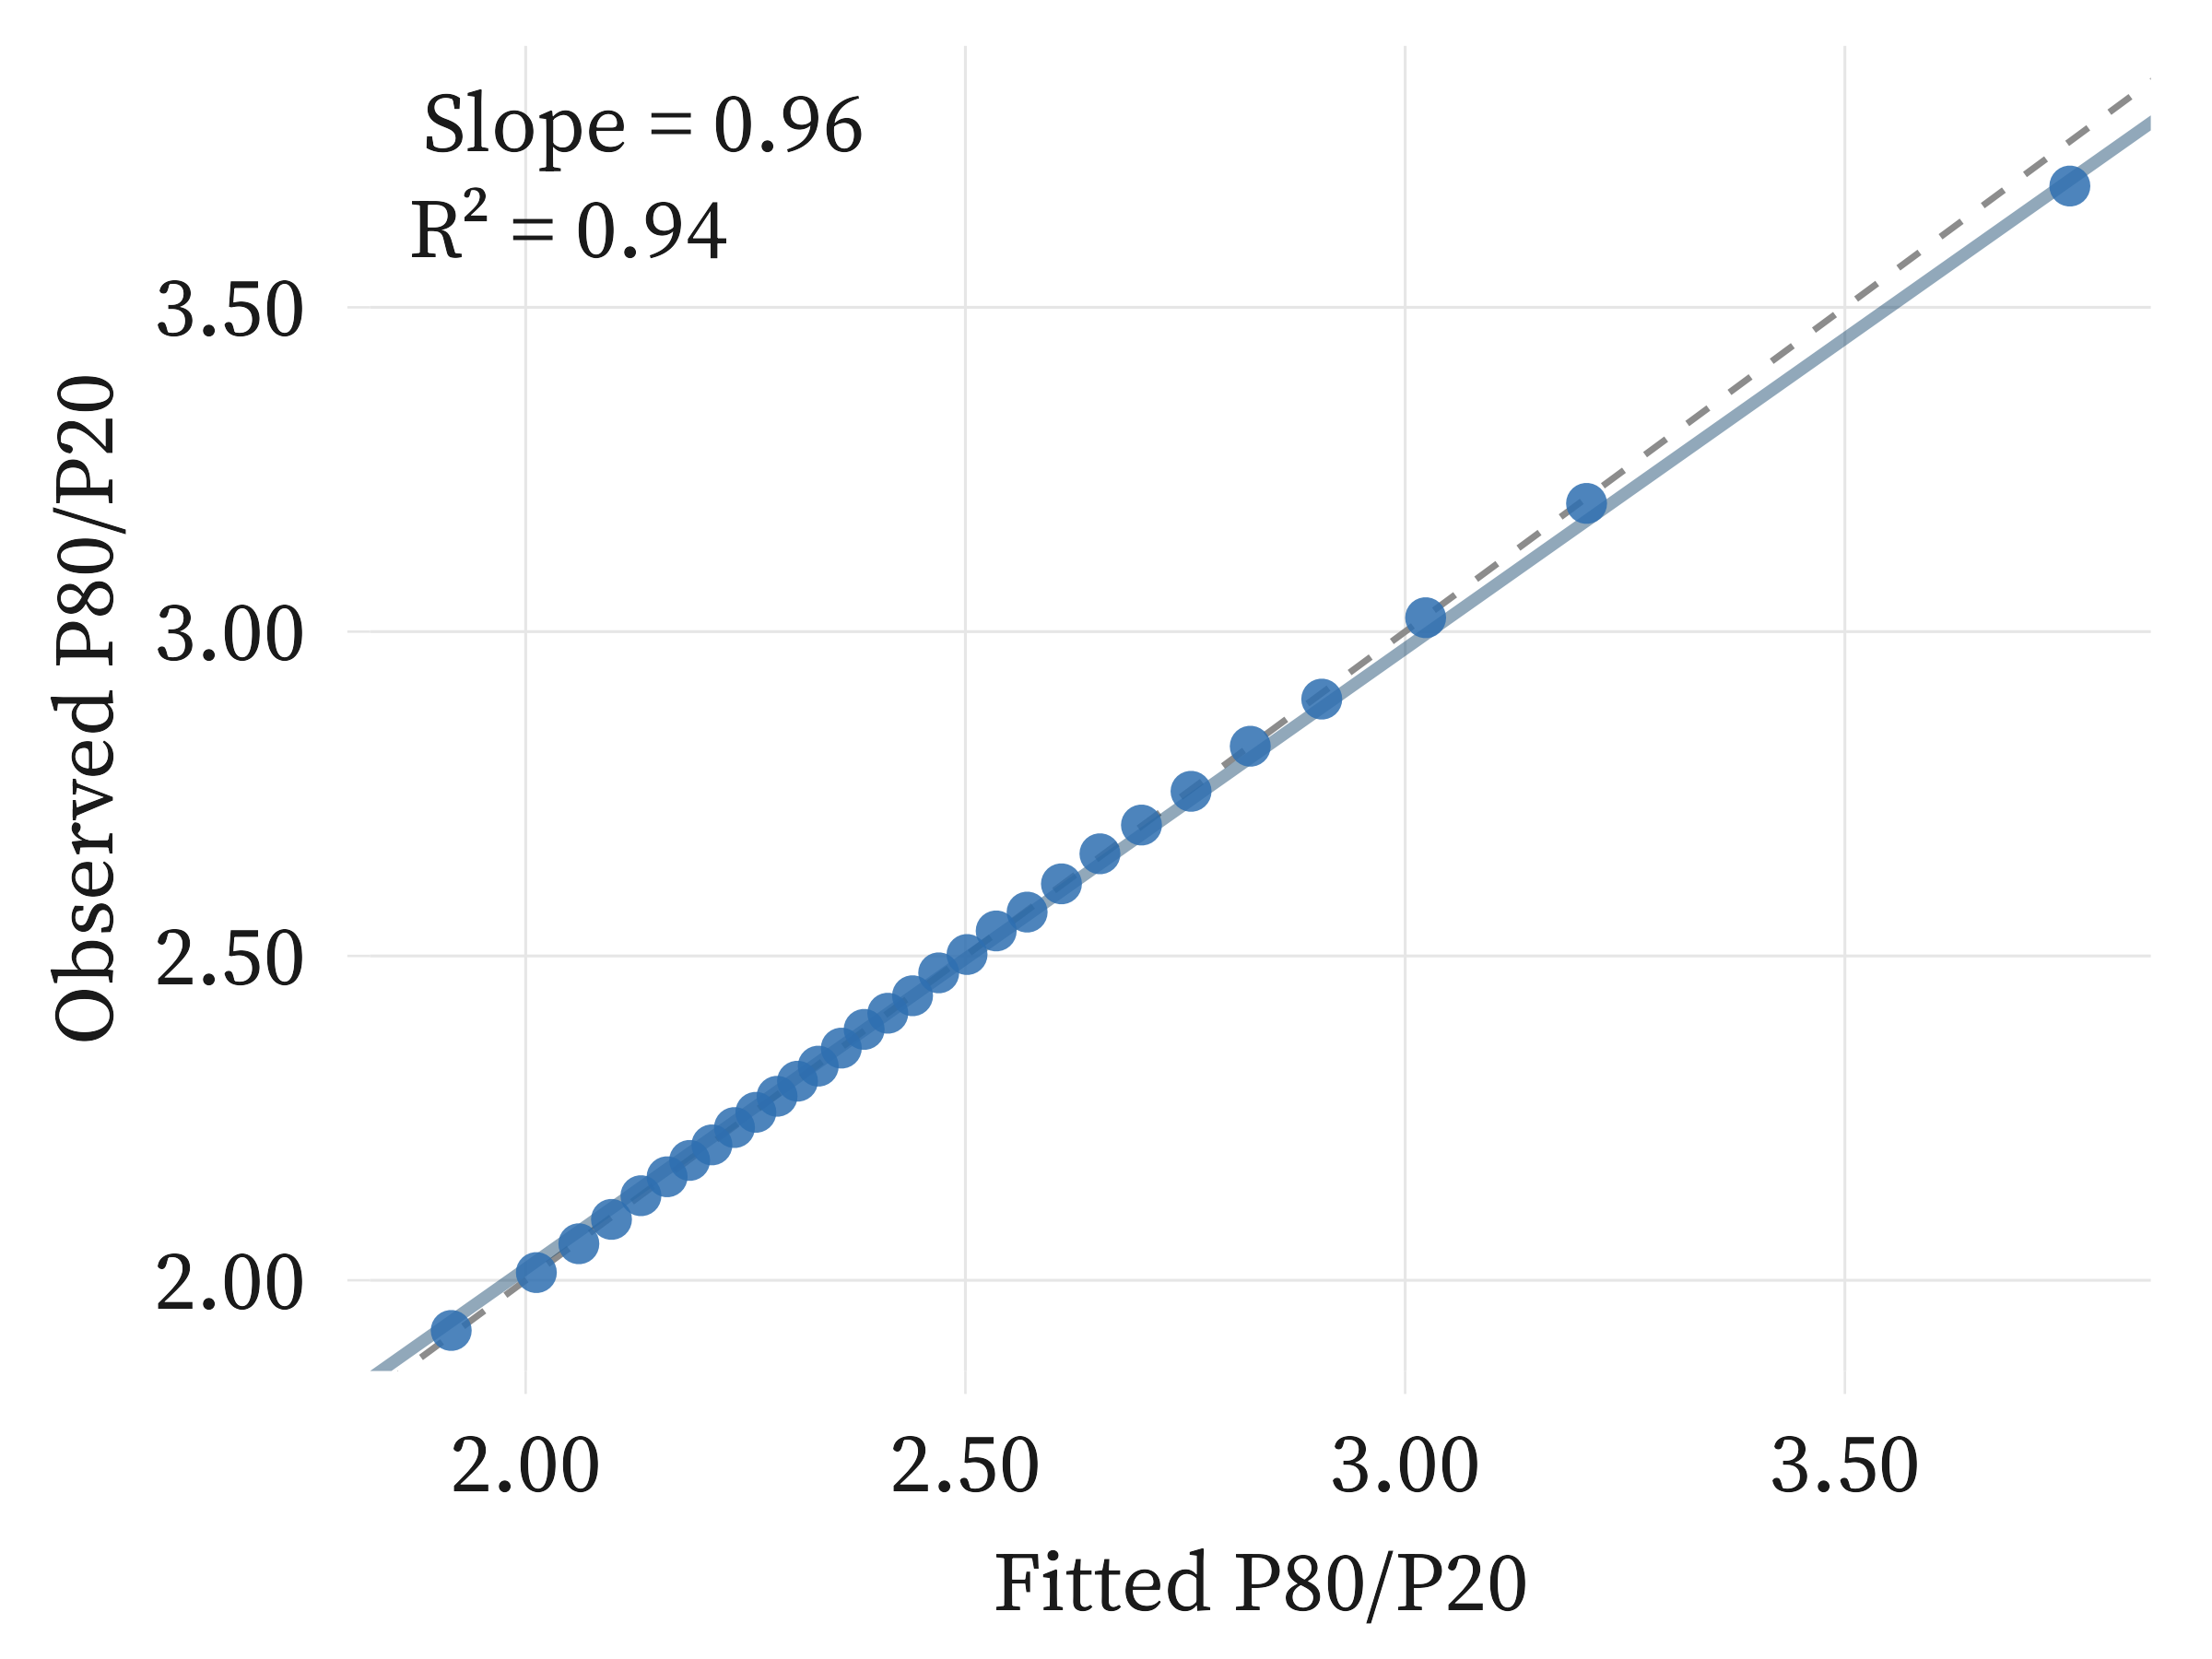
\includegraphics[width=0.55\textwidth]{output/fig_validation_p80p20.png}
\end{center}
\begin{fignotes2}
\textbf{Notes:} Binned scatter plot of the observed P80/P20 ratio of income per consumption unit against its value under the tract's fitted GB2. Tracts are grouped into 30 bins of equal population. The solid line is the population-weighted regression of observed on fitted values over all tracts; the dashed line is the 45-degree line. Source: INE, ADRH (\BaseYear{}), and author's calculations.
\end{fignotes2}
\end{figure}

\paragraph{Held-out shares} To measure how well the GB2 predicts what it is not fitted to, I refit every tract nine times, each time leaving one share out of its targets, and compare the predicted share with the published one over the tracts that publish it. The held-out shares differ from the published ones by \HoldShareMAE{} percentage points on average, between \HoldShareMAEMin{} and \HoldShareMAEMax{} depending on the share (Table \ref{tab:thresholds}, last column), against \FitShareMAE{} points when the share is part of the fit.

\subsection{Validation of the aggregate distributions}

What the app reports are percentiles of the mixtures. The mean of a mixture and its shares below income thresholds are population-weighted averages of those of its tracts, so they largely reproduce the tract fits. Its median, Gini coefficient and P80/P20 ratio are not, and the ADRH publishes them for Spain, its provinces and its municipalities; they are the main out-of-sample test of the model. Table \ref{tab:aggregate} compares them with the published values; the comparison is in \BaseYear{} euros, before the nowcast, which scales every income by the same factor.

The national median of the mixture, \texteuro\MixNatMedian{}, lies inside the published interval (\texteuro\AdrhNatMedianLo{} to \texteuro\AdrhNatMedianHi{}), \MixNatMedianErr{}\% from its midpoint. The mean, \texteuro\MixNatMean{}, differs by \MixNatMeanErr{}\% from the published \texteuro\AdrhNatMean{}. Computed as the ADRH computes it, after replacing the lowest and highest 1.5\% of incomes, the Gini coefficient of the mixture is \MixNatGini{}, against \AdrhNatGini{} published. Its P80/P20 ratio is \MixNatPEightyTwenty{}, or \MixNatPEightyTwentyBinned{} once its 20th and 80th percentiles are rounded to \texteuro 700 intervals as the published ones are, against \AdrhNatPEightyTwenty{}. The model median lies inside the published interval for \ProvMedInBinPct{}\% of provinces and for \MunMedInBinPct{}\% of the \MunValN{} municipalities with at least two tracts and published statistics (population-weighted). Gini coefficients differ from the published ones by \ProvGiniAbsErr{} points in provinces and \MunGiniAbsErr{} points in municipalities on average, and P80/P20 ratios by \ProvPAbsErr{}\% and \MunPAbsErr{}\%.

\begin{table}[H]
\centering
\begin{threeparttable}
\onehalfspacing
\caption{Model and published statistics}\label{tab:aggregate}
\footnotesize
\begin{tabular}{@{}lccc@{}}
\toprule
\textit{A. Spain} & ADRH & Model & Difference (\%) \\
\midrule
\quad Median (\texteuro) & 19,250 & 19,029 & $-$1.1 \\
\quad Mean (\texteuro) & 22,318 & 22,326 & $+$0.04 \\
\quad Gini index & 32.1 & 32.2 & $+$0.2 \\
\quad P80/P20 & 2.8 & 2.71 & $-$3.4 \\
\midrule
\textit{B. Provinces and municipalities} & Units & Mean abs.\ diff. & Mean diff. \\
\midrule
\quad Provinces: median (\%) & 52 & 0.8 & $+$0.2 \\
\quad Provinces: Gini index (points) & 52 & 0.07 & $+$0.03 \\
\quad Provinces: P80/P20 (\%) & 52 & 1.5 & $-$0.3 \\
\quad Municipalities: median (\%) & 2,253 & 0.9 & $+$0.1 \\
\quad Municipalities: Gini index (points) & 2,253 & 0.11 & $+$0.02 \\
\quad Municipalities: P80/P20 (\%) & 2,253 & 2.0 & $+$0.5 \\
\bottomrule
\end{tabular}

\begin{tablenotes}[para,flushleft]
\scriptsize
\textbf{Notes}: Statistics of income per consumption unit, in \BaseYear{} euros. Panel A compares the mixture for Spain with the totals published by the ADRH; the Gini coefficient of the mixture is computed after replacing the lowest and highest 1.5\% of incomes with the nearest remaining value, as in the ADRH. Published medians are midpoints of \texteuro 700 intervals and published P80/P20 ratios are rounded to one decimal. Panel B reports population-weighted averages of the difference between model and published statistics, in absolute value and with its sign, in per cent for medians and P80/P20 ratios and in points for Gini coefficients, for the provinces and for the municipalities with at least two census tracts and published statistics. Source: INE, ADRH, and author's calculations.
\end{tablenotes}
\end{threeparttable}
\end{table}

Table \ref{tab:thresholds} compares the shares of the population below nine thresholds that the ADRH publishes for Spain (three fixed amounts and six fractions of the national median) with those of the mixture. They differ by at most \ThrOtherMaxDiff{} percentage points, except below \texteuro 5,000, where the mixture places \ThrFiveKModel{}\% of the population against \ThrFiveKObs{}\% in the ADRH. The share of the population with the lowest incomes is thus somewhat understated: the tract GB2s cannot fully reproduce the mass of very low incomes while also matching the shares higher up.

\begin{table}[H]
\centering
\begin{threeparttable}
\onehalfspacing
\caption{Share of the population below income thresholds}\label{tab:thresholds}
\footnotesize
\begin{tabular}{@{}lcccccc@{}}
\toprule
 & & \multicolumn{3}{c}{Spain: share below (\%)} & \multicolumn{2}{c}{Tracts: MAE (pp)} \\ \cmidrule(lr){3-5} \cmidrule(l){6-7}
Threshold & \texteuro{} (2023) & ADRH & Model & Difference (pp) & Fitted & Held out \\
\midrule
Fixed amount & 5,000 & 4.3 & 3.9 & $-$0.4 & 0.69 & 0.87 \\
Fixed amount & 7,500 & 9.0 & 9.0 & 0.0 & 0.45 & 0.55 \\
40\% of the median & 7,700 & 9.5 & 9.5 & 0.0 & 0.48 & 0.58 \\
50\% of the median & 9,625 & 14.7 & 14.9 & $+$0.2 & 0.46 & 0.55 \\
Fixed amount & 10,000 & 15.8 & 16.1 & $+$0.3 & 0.47 & 0.58 \\
60\% of the median & 11,550 & 21.3 & 21.3 & 0.0 & 0.59 & 0.84 \\
140\% of the median & 26,950 & 73.6 & 73.5 & $-$0.1 & 0.46 & 0.89 \\
160\% of the median & 30,800 & 80.9 & 80.9 & 0.0 & 0.50 & 0.76 \\
200\% of the median & 38,500 & 90.0 & 89.8 & $-$0.2 & 0.47 & 0.73 \\
\bottomrule
\end{tabular}

\begin{tablenotes}[para,flushleft]
\scriptsize
\textbf{Notes}: Shares of the population with income per consumption unit below each threshold. The relative thresholds are fractions of the national median (\texteuro\AdrhNatMedian{}); for those above the median the ADRH publishes the share above, shown here as its complement. The first columns compare the shares published for Spain with those of the mixture. The last two columns are population-weighted mean absolute differences between the shares of the tracts' fitted GB2s and those the ADRH publishes for the tracts, over the tracts that publish them (\ShareTractsPopPct{}\% of the population): with every share in the fit (fitted) and with the share left out of the fit (held out). Source: INE, ADRH, and author's calculations.
\end{tablenotes}
\end{threeparttable}
\end{table}

For households, the first percentile of the mixture is \texteuro\MixPOne{}, and a household at the at-risk-of-poverty line (60\% of the median, \texteuro\ThrPovEuro{}) is placed at position \ThrPovModelP{} (Section \ref{sec:placing}), against \ThrPovObsP{} in the published distribution. At twice the median (\texteuro\ThrTopEuro{}), the mixture places \ThrTopModel{}\% of the population above, against \ThrTopObs{}\% in the ADRH.

\subsection{Decomposing income inequality}

To examine the spatial structure of inequality, I decompose the variance of log income within each autonomous community $c$ into a within-tract component and between-area components:
\begin{equation}\label{decomp}
\sigma^2_{c} =
\underbrace{\sum_{j \in c} w_j \sigma^2_{j}}_{\text{Within tracts}} +
\underbrace{\sum_{j \in c} w_j \big( \nu_{j} - \bar\nu_{k(j)} \big)^2}_{\text{Between tracts}} +
\underbrace{\sum_{k \in c} w_k \big( \bar\nu_{k} - \bar\nu_{p(k)} \big)^2}_{\text{Between municipalities}} +
\underbrace{\sum_{p \in c} w_p \big( \bar\nu_{p} - \bar\nu_{c} \big)^2}_{\text{Between provinces}},
\end{equation}
where $\nu_j$ and $\sigma_j^2$ are the mean and variance of log income in tract $j$, which for a GB2 are $\nu_j = \ln b_j + [\psi(p_j) - \psi(q_j)]/a_j$ and $\sigma_j^2 = [\psi'(p_j) + \psi'(q_j)]/a_j^2$, with $\psi$ the digamma function; $\bar\nu_k$, $\bar\nu_p$ and $\bar\nu_c$ are the population-weighted means of $\nu_j$ in municipality $k$, province $p$ and community $c$, $k(j)$ is the municipality of tract $j$ and $p(k)$ the province of municipality $k$, and $w_j$, $w_k$ and $w_p$ are population shares within $c$.

Figure \ref{fig:variance_decomp} shows the result for each community. Within-tract variation accounts for between \VdCcaaWithinMin{}\% and \VdCcaaWithinMax{}\% of the variance of log income, and for \VdCcaaWithin{}\% on average across the \VdCcaaN{} communities.\footnote{This does not contradict the homogeneity of income-generating processes within neighborhoods discussed in Section \ref{sec:method}, which refers to the mechanisms that shape incomes, such as proportional shocks, and not to the level of incomes.} Differences between tracts of the same municipality account for a further \VdCcaaTract{}\% on average, and differences between municipalities and provinces for \VdCcaaRest{}\%. For Spain as a whole, within-tract variation accounts for \VdWithin{}\% of the variance, differences between tracts within municipalities for \VdBetweenTract{}\%, between municipalities within provinces for \VdBetweenMun{}\%, between provinces within communities for \VdBetweenProv{}\% and between communities for \VdBetweenCcaa{}\%. Most inequality therefore lies within tracts, which is why the aggregate distribution depends on how incomes are distributed inside each tract and not only on tract averages. These shares rest on the fitted GB2s.

\begin{figure}[H]
\begin{center}
\caption{Decomposition of the variance of log income by autonomous community}
\label{fig:variance_decomp}
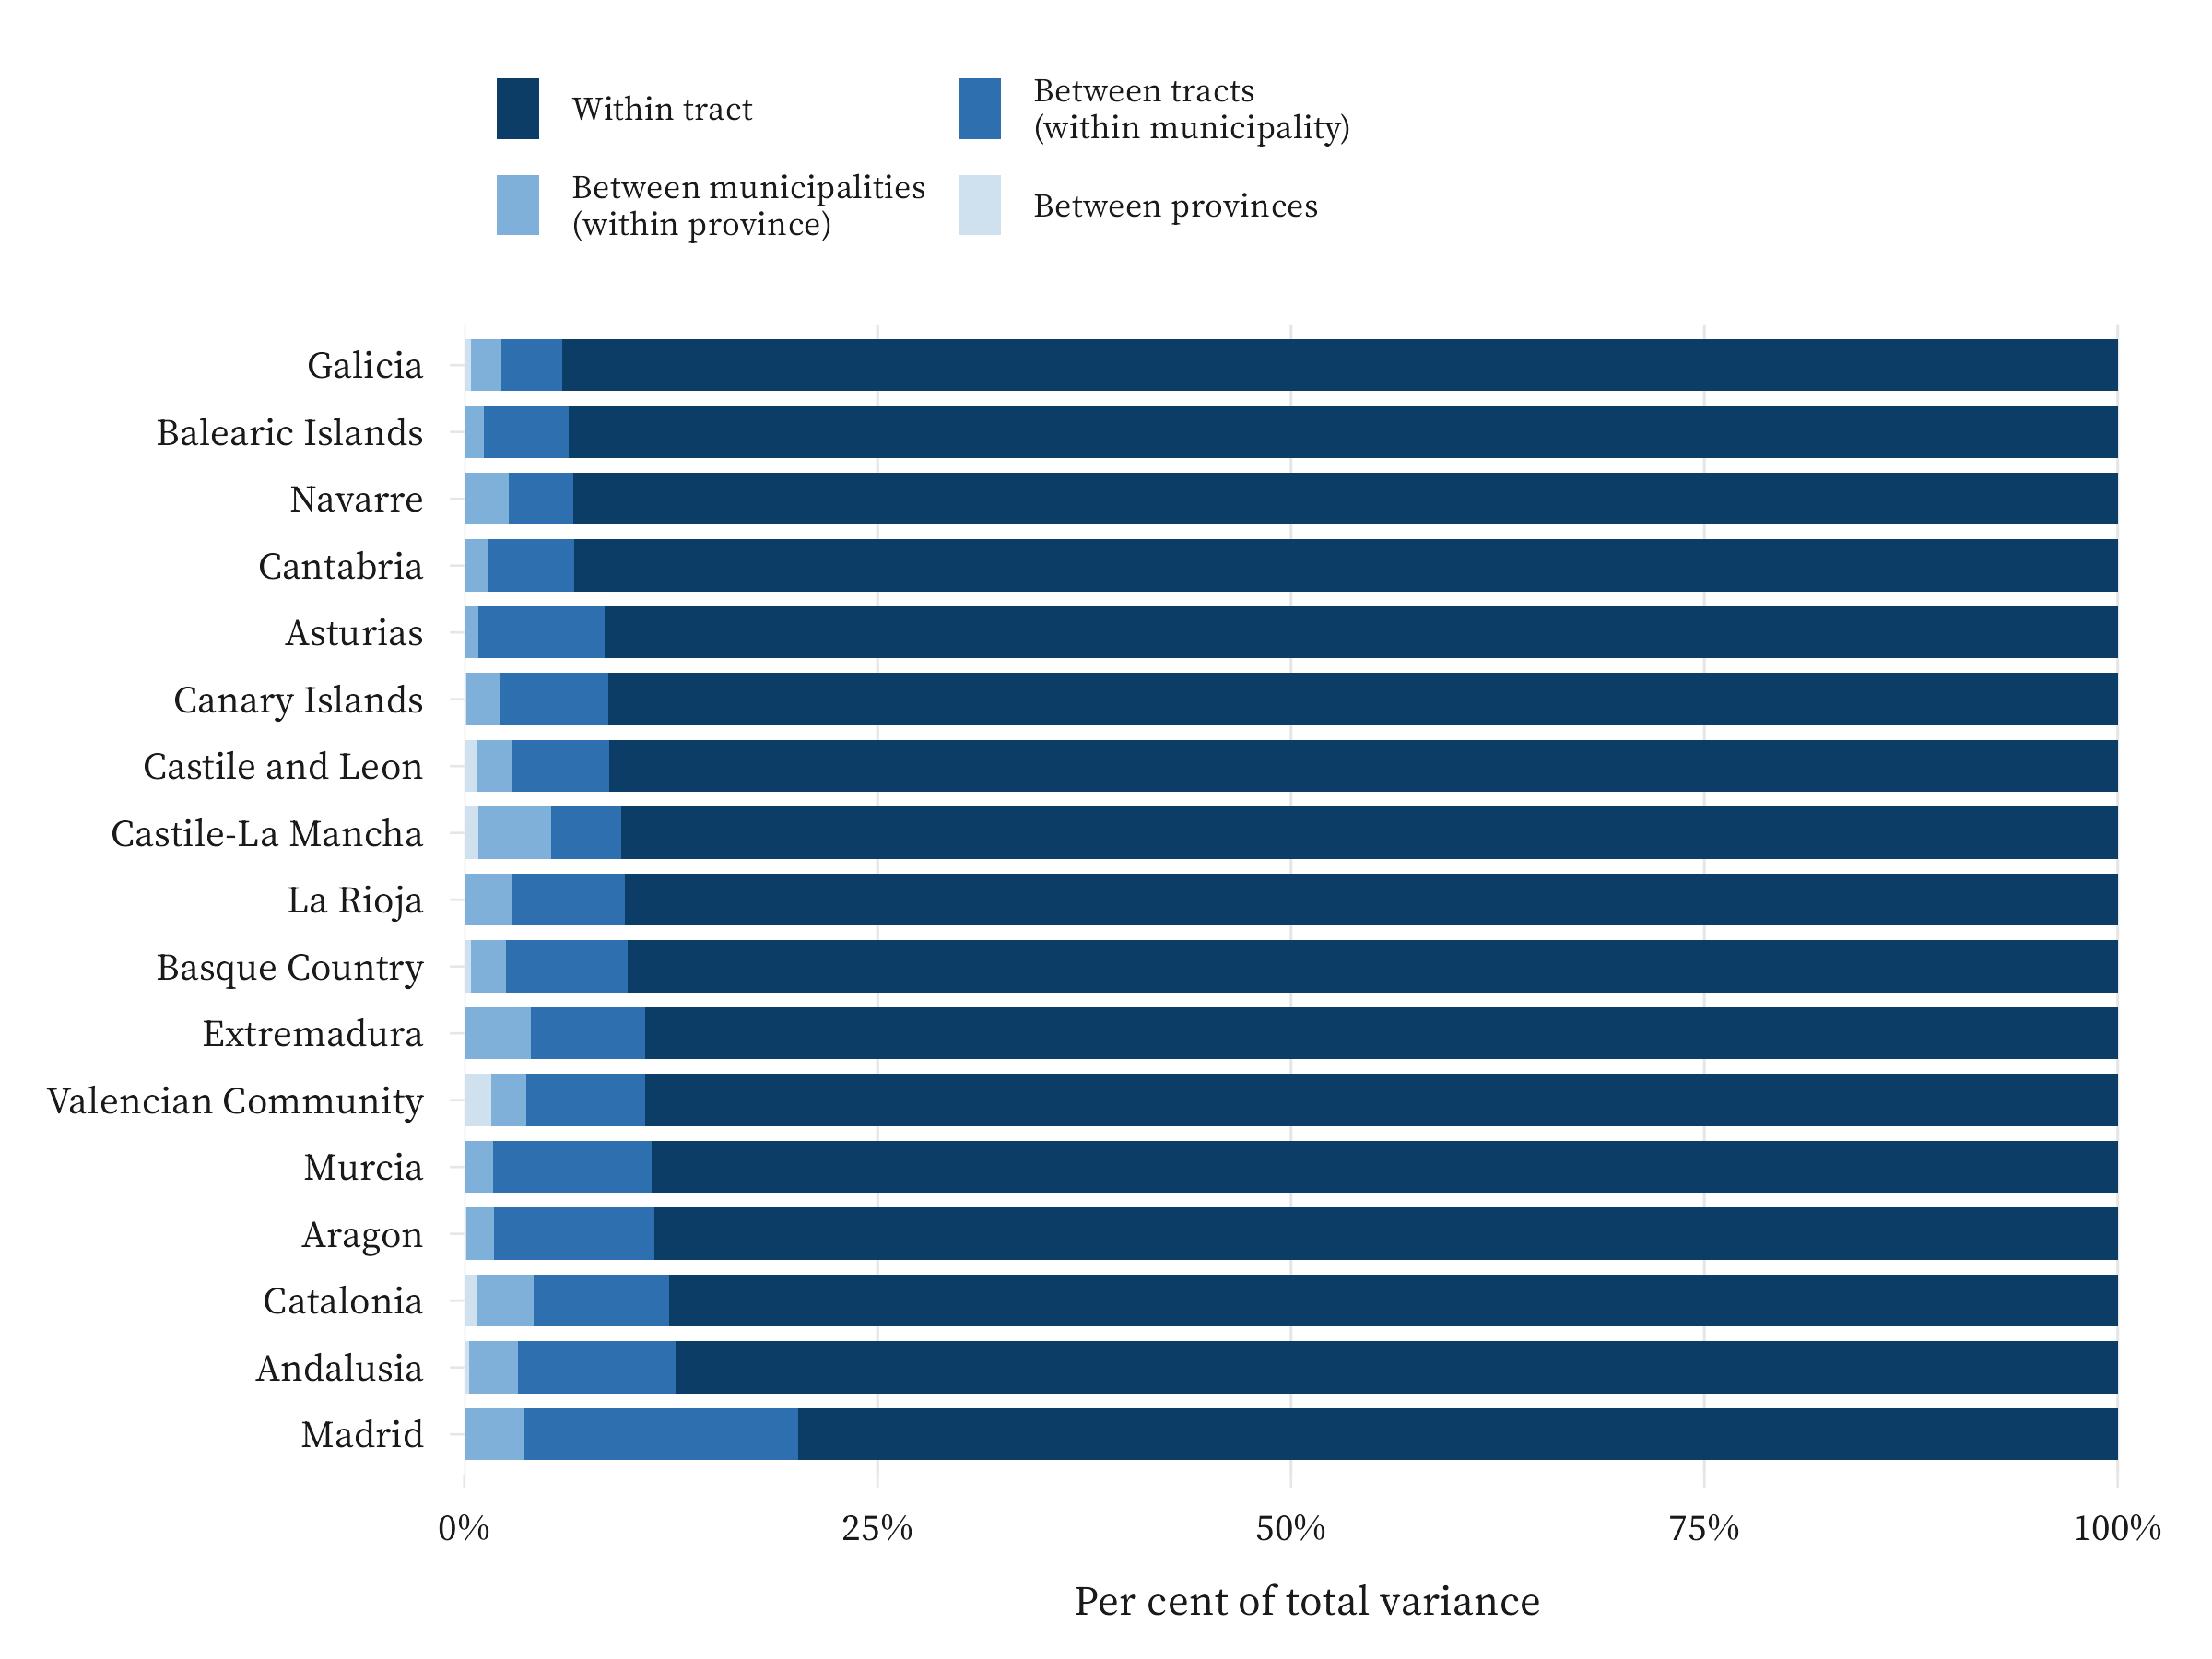
\includegraphics[width=0.85\textwidth]{output/fig_variance_decomp.png}
\end{center}
\begin{fignotes2}
\textbf{Notes:} Decomposition of equation (\ref{decomp}) for each autonomous community, excluding Ceuta and Melilla. Tracts with a GB2 fit. Source: INE, ADRH (\BaseYear{}), and author's calculations.
\end{fignotes2}
\end{figure}
